\documentclass[varwidth=28cm]{standalone}
\usepackage{tikz}
\usetikzlibrary{decorations.pathreplacing,calligraphy}
\usepackage{caption}
\usepackage{subcaption}

% To build:
% pdflatex relative_ordinal.tex
% To auto build on save:
% latexmk -pdf -pvc -halt-on-error relative_ordinal.tex
% To build png:
% convert -density 200 relative_ordinal.pdf -quality 100 -background white -alpha remove relative_ordinal.png

\def\vspacing{1.0cm}
\def\hspacing{0.4cm}
\def\overshoot{0.4cm}
\def\offset{1.2cm}

\newcommand{\abrace}[5][0.5]{
    \draw [decorate, decoration = {calligraphic brace, amplitude=5pt, aspect=#1}, very thick]
    (#2*\hspacing + \offset, -#3*\vspacing+\overshoot) --  (#2*\hspacing + \offset, -#4*\vspacing-\overshoot)
    node[right=5pt, pos=#1] {#5};
}

\newcommand{\funk}[3][black]{
    \node[left=1cm,align=right] at (0,-#2*\vspacing) {\texttt{#3}};
    \node[align=left] at (0,-#2*\vspacing) [scale=0.8,text=#1,fill=#1!5!white]
    {\texttt{def fun():} \\ \texttt{\quad \quad...}};
}

\newcommand{\elide}[1]{
    \node[minimum height=0.5cm,scale=1.5] at (0,-#1*\vspacing) {\texttt{...}};
}

\begin{document}
\begin{figure}
    % \centering
    \begin{subfigure}[t]{.37\linewidth}
        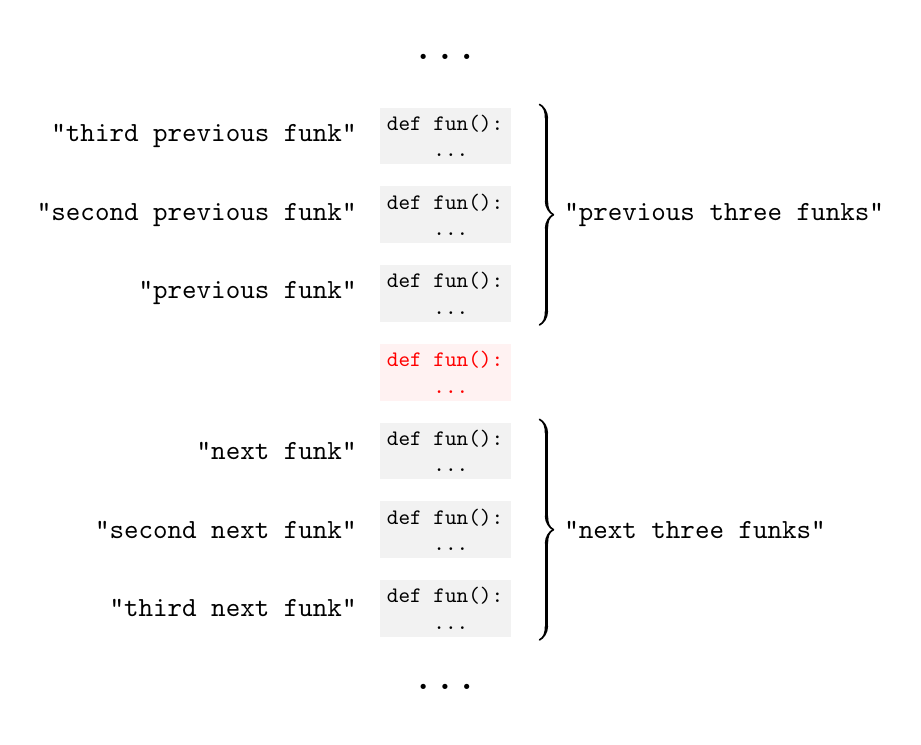
\begin{tikzpicture}
            \elide{1}
            \funk{2}{"third previous funk"}
            \funk{3}{"second previous funk"}
            \funk{4}{"previous funk"}
            \funk[red]{5}{}
            \funk{6}{"next funk"}
            \funk{7}{"second next funk"}
            \funk{8}{"third next funk"}
            \elide{9}
            \abrace{0}{6}{8}{\texttt{"next three funks"}};
            \abrace{0}{2}{4}{\texttt{"previous three funks"}};
        \end{tikzpicture}
        % \caption{Relative exclusive modifiers}
    \end{subfigure}
    \begin{subfigure}[t]{.28\linewidth}
        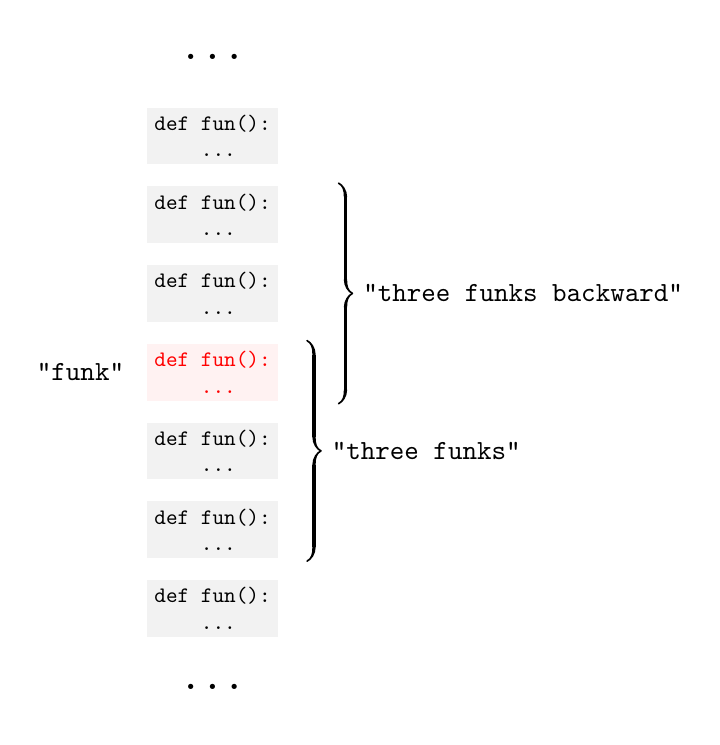
\begin{tikzpicture}
            \elide{1}
            \funk{2}{}
            \funk{3}{}
            \funk{4}{}
            \funk[red]{5}{"funk"}
            \funk{6}{}
            \funk{7}{}
            \funk{8}{}
            \elide{9}
            \abrace{0}{5}{7}{\texttt{"three funks"}};
            \abrace{1}{3}{5}{\texttt{"three funks backward"}};
        \end{tikzpicture}
        % \caption{Relative inclusive modifiers}
    \end{subfigure}
    \begin{subfigure}[t]{.3\linewidth}
        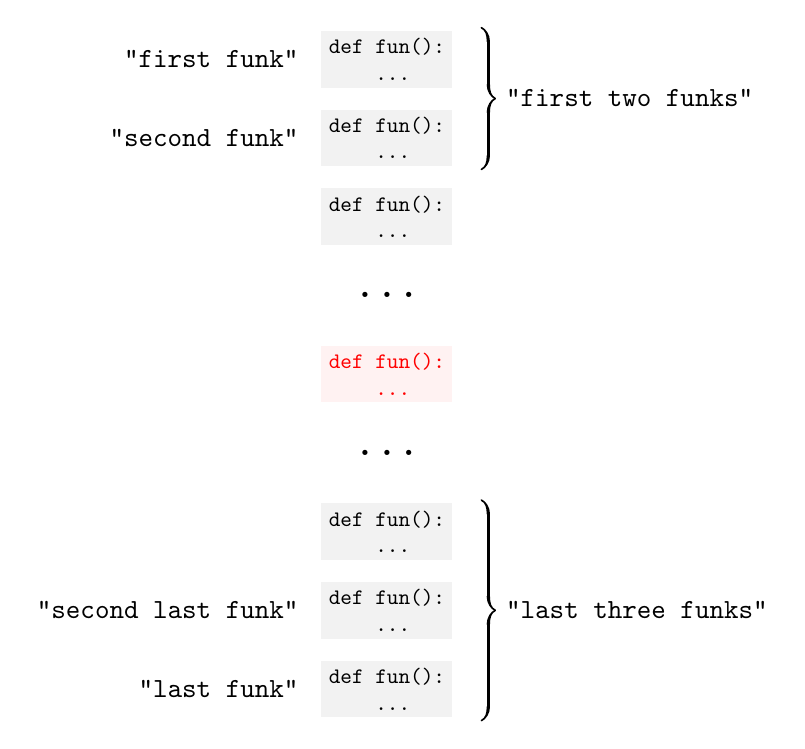
\begin{tikzpicture}
            \funk{1}{"first funk"}
            \funk{2}{"second funk"}
            \funk{3}{}
            \elide{4}
            \funk[red]{5}{}
            \elide{6}
            \funk{7}{}
            \funk{8}{"second last funk"}
            \funk{9}{"last funk"}
            \abrace{0}{7}{9}{\texttt{"last three funks"}};
            \abrace{0}{1}{2}{\texttt{"first two funks"}};
        \end{tikzpicture}
        % \caption{Absolute modifiers}
    \end{subfigure}
    \\
    \begin{subfigure}[t]{\linewidth}
        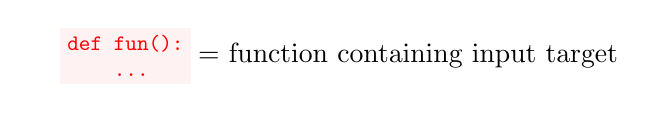
\begin{tikzpicture}
            \funk[red]{0}{}
            \node[align=left,right=0.8cm] at (0,0) {= function containing input target};
        \end{tikzpicture}
    \end{subfigure}
    \\
    \begin{subfigure}[t]{\linewidth}
        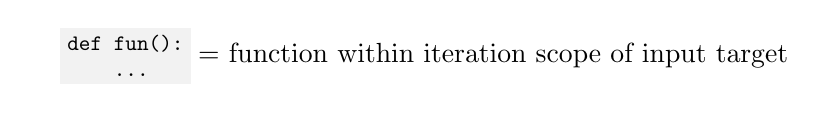
\begin{tikzpicture}
            \funk{0}{}
            \node[align=left,right=0.8cm] at (0,0) {= function within iteration scope of input target};
        \end{tikzpicture}
    \end{subfigure}

\end{figure}
\end{document}
